\documentclass[conference]{IEEEtran}

\usepackage[dvipdfmx]{graphicx}

\usepackage{bm}

\usepackage[fleqn]{amsmath}
\usepackage{amssymb}
\usepackage{url}
\usepackage{multirow}
\usepackage{caption}
\usepackage{subcaption}
\captionsetup{compatibility=false}

\newlength{\graphwidth}

\newcommand{\birth}[1]{\mathcal{C}(#1)}
\newcommand{\distinct}[1]{\mathcal{N}_n^d(#1)}
\newcommand{\distinctnnn}[1]{\mathcal{N}_3^d(#1)}

\hyphenation{op-tical net-works semi-conduc-tor}

\begin{document}

\title{Identifying the Applied Obfuscation Method towards De-obfuscation}
% \title{Identified method of applied obfuscation for de-obfuscation}

% author names and affiliations
% use a multiple column layout for up to three different
% affiliations
\author{\IEEEauthorblockN{Hayato Sagisaka}
  \IEEEauthorblockA{Division of Frontier Informatics,\\
    Graduate School of Kyoto Sangyo University.}
\and
\IEEEauthorblockN{Haruaki Tamada}
\IEEEauthorblockA{
  Faculty of Computer Science and Engineering,\\
  Kyoto Sangyo University.}
}

\maketitle

% As a general rule, do not put math, special symbols or citations
% in the abstract
\begin{abstract}
  Recently, to prevent cracking, the various protection methods have
  been proposed.  One of the protection methods is the obfuscation
  method. Obfuscation method changes the program into hard to
  understand for hiding secret information in the program.
  %%%
  On the other hand, de-obfuscation is an interesting research topic
  for protecting the software.  Since, though vulnerable protection
  methods are dangerous, measuring the robustness of the method was not
  discussed.
  %%%
  In this paper, we tackle to identify the applied obfuscation methods
  towards de-obfuscation.  To perform de-obfuscation requires a
  suitable method for each obfuscation method.  For this, we
  obfuscated programs by two practical tools and three algorithms from
  one academic tool.  Then, we analyzed the programs and extracted
  characteristics from them based on opcodes.  By using the proposed
  method, we could identify the applied obfuscation method.
  % Recently, illegalities are increasing with the spread of software.
  % For the measures, there are methods of protect called obfuscation.
  % The obfuscation is method to do difficulty for analyzing to
  % program.  On the other hand, there is de-obfuscation that return
  % obfuscated program into former program.  De-change as different
  % method is to break the programs, it is necessary to identify that
  % obfuscation is applied to do de-obfuscation.  In this paper, we
  % measure find easy methods of protection by measuring to identify
  % easy method of protection.  Exactly, we analyze the obfuscated
  % programs and find the characteristic of obfuscation method.  Then,
  % we inspect that exacted characteristic is effective method for
  % unknown products and obfuscation methods.
\end{abstract}

% no keywords

% For peer review papers, you can put extra information on the cover
% page as needed:
% \ifCLASSOPTIONpeerreview
% \begin{center} \bfseries EDICS Category: 3-BBND \end{center}
% \fi
%
% For peerreview papers, this IEEEtran command inserts a page break and
% creates the second title. It will be ignored for other modes.
\IEEEpeerreviewmaketitle

\section{Introduction}\label{sect:introduction}

Serious security incidents have arisen, such as illegal analysis and
software theft.  To prevent such malicious attacks, many protection
methods were proposed.  However, the robustness of the protection
methods were never discussed.  Increasing the robustness needs a more
deeper discussion about robustnesses and vulnerabilities.  Especially,
systematizing how to attack to the protection methods helps evaluation
and construction of more robust protection method.

This paper focuses on de-obfuscation which converts an obfuscated program
to more understandable program.  If strong de-obfuscation method is
established, fragile obfuscation methods will be gone.
%
We consider the process to apply the de-obfuscation method.
%
To get the de-obfuscated program, we apply the reverse transformation
of the obfuscation algorithm.  The each obfuscation method have
different algorithm.  That is, reverse transformation also proper for
each obfuscation method.  Therefore, in the first step, we must
identify the applied obfuscation method in order to de-obfuscate.
This paper proposes the identifying method for the applied obfuscation
method towards de-obfuscation.

We develop three research questions to evaluate the proposed method.
\begin{description}
\item[RQ1]   What characteristics does the obfuscation method have?
\item[RQ2-1] Are the characteristics useful to identify the known
  obfuscation method applied to an unknown product?
\item[RQ2-2] Are the characteristics useful to identify the unknown
  obfuscation method applied to known product?
\end{description}
We conducted the empirical studies to answer the above research
questions.  The result of the studies shows that the proposed method
could identify the applied obfuscation method based on the survey of
the obfuscation methods in advance.

The remainder of this paper is organized as following.
%
Section \ref{sect:relatedworks} reviewed related works.
%
Section \ref{sect:method} describes the proposed method and illustrates
its process.
%
Section \ref{sect:studies} presents the empirical studies to answer the
research questions.
%
Section \ref{sect:conclusion} shows conclusion and some future works.


% Recently, illegalities such as illegality access and analysis are
% increasing.  Various methods of protection in software are proposed
% as a measure.  Method of protection in software can guard from the
% injustice access and analysis by prevent the program in advance.
% There is a method of protection called obfuscation that is one of
% the method of protection in software.  The obfuscation is method of
% protection so as not to analyze program.
%%%
% For example, name obfuscation that is to change unknown name of
% meaning into class name and method name and control flow of
% obfuscation that is to generate code that is not able to understand
% the meaning when de-compile is tried to do are proposed various
% methods how we falsify data so as not to analyze.  There are the
% methods called de-obfuscation that is to return obfuscation program
% to original program.  As de-obfuscation is taken by illegality
% access, the measure is need.  We consider useful in analyzing for
% malware that is protecting obfuscation by doing research to
% de-obfuscation.  So, we consider new measure for obfuscation and
% discussion about vulnerability of obfuscation.  However, the
% research about de-obfuscation do not ever take for the present.  For
% taking the de-obfuscation, it takes to identify the used obfuscation
% from various obfuscation and needs to make sure how to analyze.
% Then, in this paper, we analyze the obfuscated program and search
% the characteristic of method of obfuscation.  In specific, we
% analyze the command of software ( jar file ) that is applied method
% of obfuscation, and get to estimation of creation in each n-gram of
% opcode as preliminary experiment.  We compare their results and
% extract characteristic.  After that, we inspect the efficiency for
% unknown product and unknown method of obfuscation from extracted
% characteristic as evaluation experiment.

\section{Related Work}\label{sect:relatedworks}

The previous protection methods are categorized into (1) preventing
the theft techniques, (2) detecting stolen programs, and (3) proving
the theft\cite{collberg09surreptitious}.
%
In category (1), there were proposed obfuscation methods, and
anti-assemble methods\cite{tyma00patent,monden97ieice}.  Also,
category (2) includes software birthmark
methods\cite{tamada04iasted,tamada05ieice}, and category (3) includes
software watermark methods\cite{collberg99popl}.

An attack method against obfuscation methods were proposed for
category (1)\cite{cimato05jss}.
%
Cimato et al. proposed the conversion method to de-obfuscate the names
in a program.
%
Blanc et al. also proposed the de-obfuscating the program to clarify
its control flow with abstract syntax tree\cite{preda06amast}.

Both methods are quite important, since those methods become one of
technique to evaluate the robustness and vulnerabilities of the
obfuscation methods.  However, to perform de-obfuscation requires a
suitable method for each obfuscation method.  Futhermore, the applied
protection methods are generally private information.  Therefore,
identifying applied protection methods are important to the first step
of the de-obfuscation.

% Method of protection in software can separate methods into three
% technique groups that is (1) prevention of plagiarism, (2) detection
% of plagiarism, and (3) identification of
% plagiarism.\cite{collberg09surreptitious} (1) as obfuscation methods
% and anti-de-assemble methods\cite{tyma00patent,monden97ieice}, (2) as
% bath mark in software methods\cite{tamada05ieice},and (3) as watermark
% in software methods mainly researched\cite{collberg99popl}.
% 
% Methods of attack are proposed for obfuscation with a factor technique
% of (1).  One of them is de-change for name obfuscation that is to
% change the variable name and function name into programs for hard
% reading\cite{cimato05jss}.  The other one is to classify method for
% using the abstract syntax tree for applied program with obfuscation
% method that is to complicate the control flow.  Both methods are
% useful to establish as methods of attack.  On the other hand, for
% specializing obfuscation, the method is not general.  Established
% methods of attack that are bath mark that are a factor technique of
% (2) and (3) and watermark do not exist.  However, base mark and
% watermark have common points that is to use the information in
% program.  That is to say, as their methods are to change the
% information in reference program, these methods will become to the
% methods of attack.  For that reason, obfuscation methods with a factor
% technique of (1) is used as methods of attack\cite{tian13hpcc}.  On
% the other hand, the methods that is to evaluate unnatural from methods
% of protect as method of evaluation with obfuscations are
% proposed\cite{kanzaki14ipsj}.  There is method that is to estimate
% unnatural from methods of protect by the probability of creations that
% is to abstract n-gram from opcode in programs.  Kanzaki's method is to
% evaluate the artificial of degree between opcode that is applied by
% method of protection and opcode that is to do output by compiler.

\section{Proposed method}\label{sect:method}

\subsection{Key Idea}

Various obfuscation methods are proposed in a few decade.  Almost
methods convert the given program in order to hide the private
information in the program.  Each coversion characterize the
obfuscation algorithm to hide a certain information.
%
For example, name obfuscation hide means of variables, methods, and
class names by changing meaningless names\cite{tyma00patent}.
Because, we assume that the names in the program greatly help to
understand the program.  Threfore, the name obfuscation method
protects the program by converting to more incomprehensible program.
Some algorithms are proposed in the name obfuscation methods how to
change the names.

Straightforward algorithm is to change variable names into one
alphabet characters.  More powerful algorithm changes variable names
into reserved words, and invisible characters such as spaces, tabs,
control sequences, and etc\cite{dasho}.  Other algorithms change
method names to introduce overloading\cite{tyma00patent}, and change
not definition parts of symbol names, but use parts with dynamic name
resolution mechanism\cite{tamada07ieice,tamada08iasted}.

Even though the obfuscation algorithms categorized into the name
obfuscation methods, we will acquire characteristics of each algorithm
from the conversion process and resultant programs.
%
Similarly, the case of using other protection methods, characteristics
of the method will arise.  Therefore, we tackle to identify the
applied obfuscation method towards de-obfuscation by measuring the
program artificiality.

% As Methods of protection have various methods, various methods carry
% out the change of program.  The change is carried out the
% characteristic management to hide the informations that are to notice
% various methods.  For example, as the name in program ( a variable
% name, method name, and class name etc ) have meaning to contribute for
% understanding program, name obfuscation\cite{tyma00patent} protects
% program to change the name that is difficult and no-meaning.  This
% obfuscation methods are gotten characteristic by methods that is to
% change the every name.
% 
% The name obfuscations such as method that the name is changed one of
% alphabet, invisibility word such as space and tab, reserved name,
% repeat name\cite{dasho}, and not only definition part of name but also
% using part of hiding are proposed various methods\cite{tamada07ieice}.
% 
% However, as these name obfuscation carried out obfuscation, it become
% to be seen the characteristic that is to see various methods to name
% in program.  That is to say, the case of name obfuscation is able to
% identify that every name obfuscation is applied by observing the name.
% Even other method of protect, they are able to hope to be reflected
% the characteristics of method of protect to program in after change.
% So, we try to identify method of obfuscation by analyzing
% characteristic of program in after change.

\subsection{Overview of the Proposed Method}

\begin{figure}[b]
  \centering
  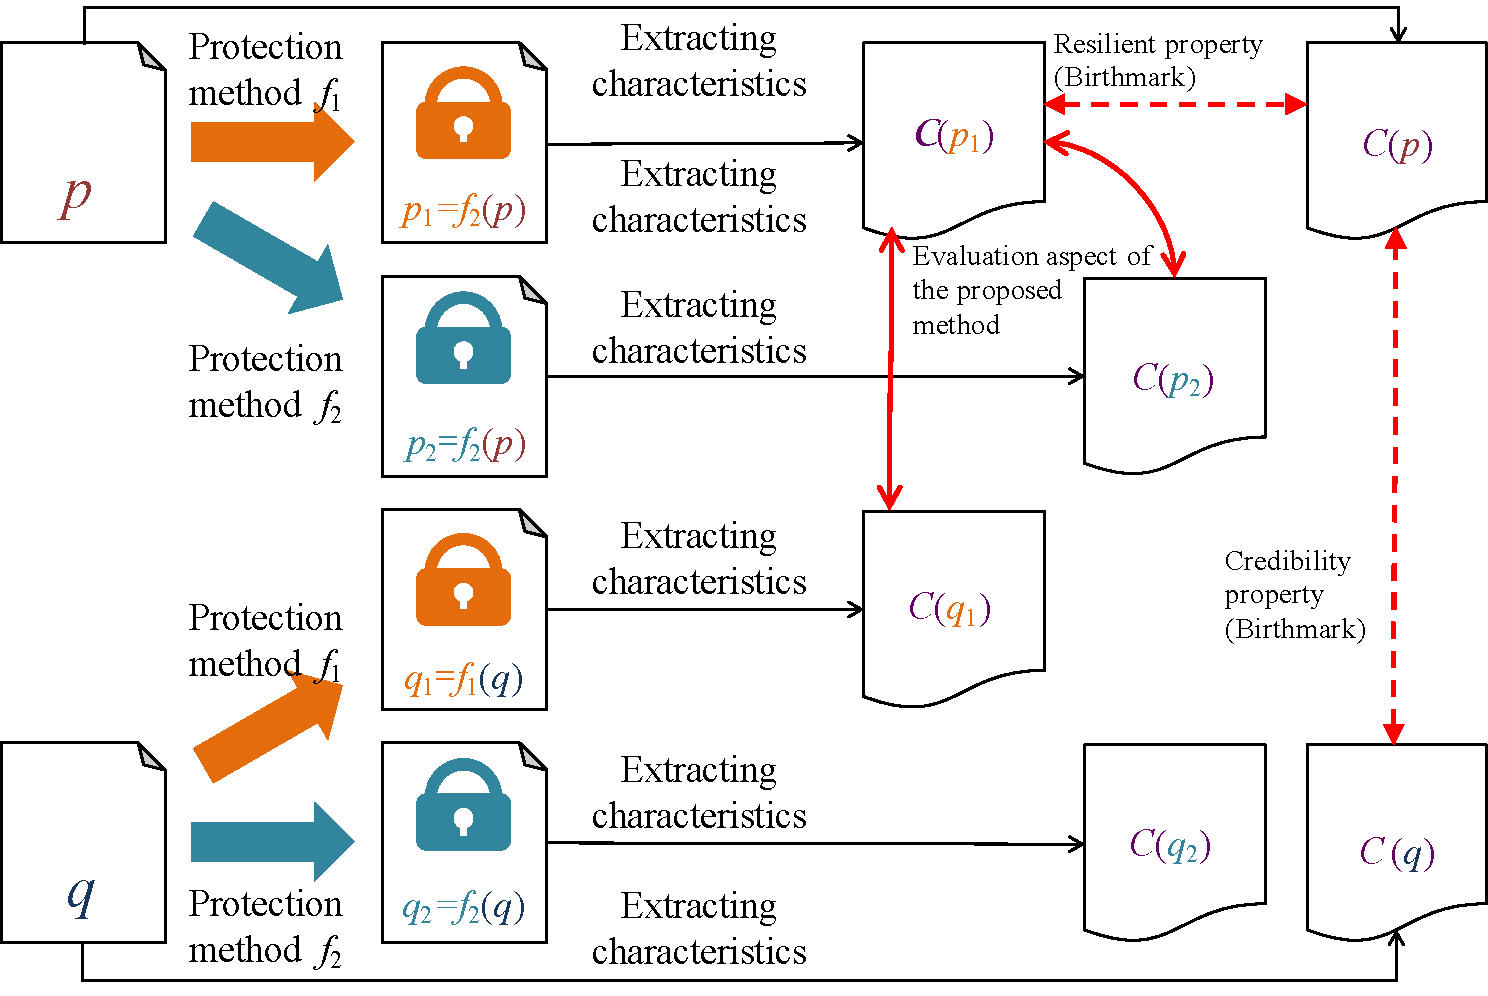
\includegraphics[width=0.49\textwidth]{images/key_idea}
  \caption{Key idea of the proposed method}\label{fig:keyidea}
\end{figure}

The birthmark methods have been proposed, which use characteristics of
the program\cite{tamada04iasted,tamada05ieice}.  Birthmark method
originally computes similarities between the programs with the
extracted native characteristics in order to detect pirated programs.
%
The process of the proposed method is ported from birthmark methods,
which is to extract the characteristics of the program, and to compare
them.  However, extracting characteristics are absolutely different.
The birthmark methods focus on the characteristics of the program.
The proposed method focuses on the characteristics of the protection
method.

On the other hands, Kanzaki et al. proposed the method to measure the
stealthiness of the program\cite{kanzaki14ipsj}. The method extracts
$n$-gram from the opcodes of the given program, and computes
artificiality by the probability from the corpus.  The artificiality
means how {\em natural} opcode sequences are in the target program.
Kanzaki et al. assume that a compiler generates natural opcode
sequences.  Generally, protection methods alter the opcode sequence by
their algorithm.  Then, the protected program may have unnatural
opcode sequences.  If a protection method has {\em natural} opcode
sequences, the algorithm of the method is stealthy.

We focus on the method to compute artificiality, and assume that
protected program have a certain characteristics of the protection
algorithm.  Then, we tackle to identify the protection method of the
program by the extracted characteristics.

Figure \ref{fig:keyidea} shows the key idea of the proposed method.
In the figure \ref{fig:keyidea}, we acquire obfuscatd program $p_1$
and $p_2$ from original program $p$ by certain obfuscation algorithm
$f_1$ and $f_2$ ($p_1 = f_1(p), p_2 = f_2(p)$).  Then, using
characteristics extraction function $\mathcal{C}$, we extract certain
characteristics $\birth{p}$, $\birth{p_1}$, and $\birth{p_2}$ from
$p$, $p_1$, and $p_2$.

The evaluation aspects of the birthmark method are resilient property
and credibility property.  To evaluate resilient property compares
$\birth{p}$ and $\birth{p_1}$, then the high score shows that $p_1$
and $p$ are in the copy relation.  Also, credibility property compares
$\birth{p}$ and $\birth{q}$, then the low score shows that $p$ and $q$
are developed independently.

The evaluation aspect of the proposed method is $\birth{p_1}$ and
$\birth{p_2}$, and $\birth{p_1}$ and $\birth{q_1}$.  A low score
between former relation ($\birth{p_1}$ and $\birth{p_2}$) shows
different protection methods were applied.  Also, high score between
latter relation ($\birth{p_1}$ and $\birth{q_1}$) shows the same
protection method was applied.

% Base mark that is to distinguish others programs by characteristic in
% program is proposed\cite{tamada05ieice}.  Base mark is technique that
% is to find plagiarism by comparing characteristic with ones that
% program have originally.  For difference purpose from this research,
% it can not apply the base mark as it is, but it can expect the advance
% method of base mark as standard way of comparison.
% 
% Kanzaki's propose method that is to evaluate unnatural of
% program\cite{kanzaki14ipsj}.  This program is to expect n-gram from
% opcode in program and to evaluate unnatural by requiring generative
% probability.  For example, Matuda's evaluate difficult discovery of
% method of protection by comparing unnatural of fragment of
% code\cite{matsuda15ipsj}.
% 
% We assume that method of protection have a proper characteristic by
% forcing on this method.  Thus, for proper characteristic, we try to
% identify how method of protection are used.  If method of protection
% can be identified, specializing method of attack for and attack for
% the method of protection understanding to method of protection are
% possible.  Conversely, if method of protection can not be identified,
% the key of attack can not be taken and attack is difficult.

% It show a schematic diagram of method of protection at
% Figure\ref{fig:keyidea}.  Process method and base mark are same as
% processing that is to extract characteristic from protected program.
% On the other hand, evaluation point are different.
%%%% 
% %式が出るので後
%%%% 
% In Figure\ref{fig:keyidea}, protected program $p_1=f_1(p)$,
% $p_2=f_2(p)$ are gotten by any methods of protection $f_1$ と $f_2$
% with program $p$.
%%% 
% So, any characteristics $\birth{p_1}, \birth{p_1}, and \birth{p_2}$
% are gotten from $p, p_1, p_2$ , for using the feature extraction
% function$\mathcal{C}$.
%%% 
% The interest in base mark technology is part of showing a arrow by a
% dotted line in Figure\ref{fig:keyidea}.  As a result, we evaluate
% that how do $\birth{p}$, $\birth{p_1}, and \birth{p_2}$ look like?,
% and how do $\birth{p}$ and $\birth{q}$ look difference?
%%% 
% The interest in proposed method is part of showing a arrow by a
% solid line in Figure\ref{fig:keyidea}.  That is to say, we compare
% that how do protected same programs by different method look
% difference ($\birth{p_1}$と$\birth{p_2}$)? and how do protected
% different programs by same method look like?

\subsection{Characteristics of the Proposed Method}\label{sect:artificiality}

To implement the proposed method, almost birthmark methods would fail
to identify the protection method.  Because, if we apply a certain
protection method $f_1$ to different programs $p$ and $q$, birthmark
method expects $\birth{p} \neq \birth{q}$.  However, the proposed
method expects $\birth{p_1} \approx \birth{q_1}$.

We focus on the artificiality evaluation method by Kanzaki et al. to
the proposed method.  A certain protection method inserts ridiculous
opcode sequence into never executed block.  Another certain protection
method changes the natural opcode sequence to unnatural one.  Such
unnatual opcode sequence might be the characteristics of the
protection method.

Originally, Kanzaki et al. computed the artificiality by probability.
Ohtaki et al. ported Kanzaki's method for an object oriented language,
such as Java\cite{gekka14scis}.  The method uses perplexity metric
instead of Kanzaki's probability for computing the artificiality.  The
perplexity metric shows the complexity of the natural language.  Low
perplexity means that the next word is easy to expect.

On the other hand, a certain protection method duplicates original
natural opcode sequence.  Such duplicated sequence is still natural.
Therefore, we also focus on the frequencies of the $n$-gram.

Then, we employ the perplexity metric and frequency of the $n$-gram as
the characteristics of the protection method.

% Although Extracting characteristic is like base mark in method, it do
% not carry out as expected to itself.
% %式が出るので後
% 
% Because, in protected different program $p$ and $q$ by same method
% $f_1$, as base mark is that program itself is to difference, we expect
% result as difference($\birth{p_1} \neq\birth{q_1}$).  However, as
% proposed method is to take the characteristic in method of protection
% itself, we expect result as same($\birth{p_1} \approx \birth{q_1}$).
% 
% Therefore, we observe Kanzaki's propose method that is to evaluate
% unnatural of program\cite{kanzaki14ipsj}
% 
% This method is to use the rare in $n$-gram of opcode.  In method of
% protection, the case is absolutely to insert the sequence of orders in
% place that is not carried out impossibility, and other case is to
% rearrange rare order as understanding in original order is difficult.
% 
% Thus, we can judgment whether rare order is true or false as showing
% rarity.  it is to say that these rare order is characteristic in
% method of protection.  creation probability use the
% perplexity\cite{gekka14scis}.  Perplexity is known average branch and
% ais index that express complexity as language.  It is express that the
% more little this value is,the more next coming language is predicted.
% As a result, it is say that the more little the value is, the more
% natural value is.
% 
% On the other hand, in the method of protection, the case is that the
% compiler outputted original orders with repeated.
% 
% As The original order is difference with use frequency, it is not to
% say the rare.  Thus, the only creation probability is not able to
% observe the characteristic in method of protection.  Therefor, we
% observe the frequency in $n$-gram.
% 
% In the above, we extract order in $n$-gram from program, and are
% characteristic in method of protection with the rare ( perplexity )
% and frequency.

\section{Empirical Studies}\label{sect:studies}

\subsection{Overview}\label{sect:study_overview}

\begin{figure*}[bt]
  \centering
  \setlength{\graphwidth}{0.32\textwidth}
  \begin{minipage}[b]{\graphwidth}
    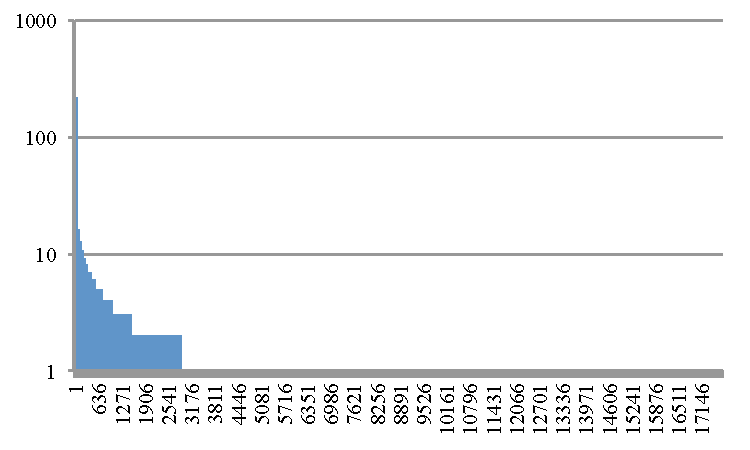
\includegraphics[clip,width=1.0\columnwidth]{images/ORI_ASM}%
    \subcaption{Original ASM}
    \label{fig:asm-5gram-original-histogram}%
  \end{minipage}
  \hfill
  \begin{minipage}[b]{\graphwidth}
    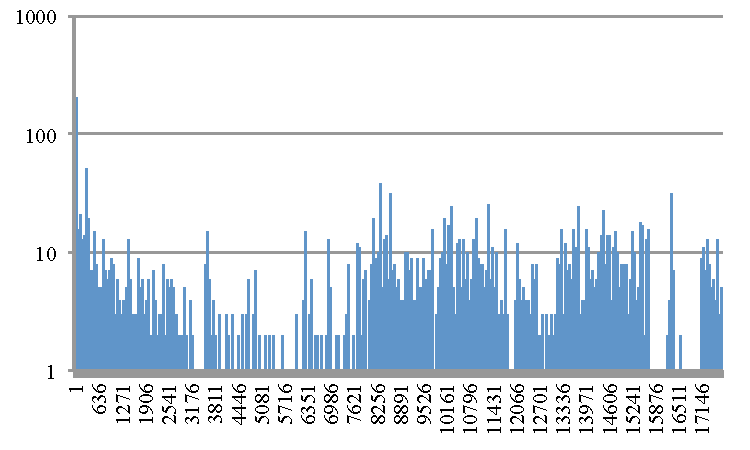
\includegraphics[clip,width=1.0\columnwidth]{images/ALL_ASM}%
    \subcaption{ALL (Allatori Java Obfuscator)}\label{fig:asm-5gram-ALL-histogram}%
  \end{minipage}
  \hfill
  \begin{minipage}[b]{\graphwidth}
    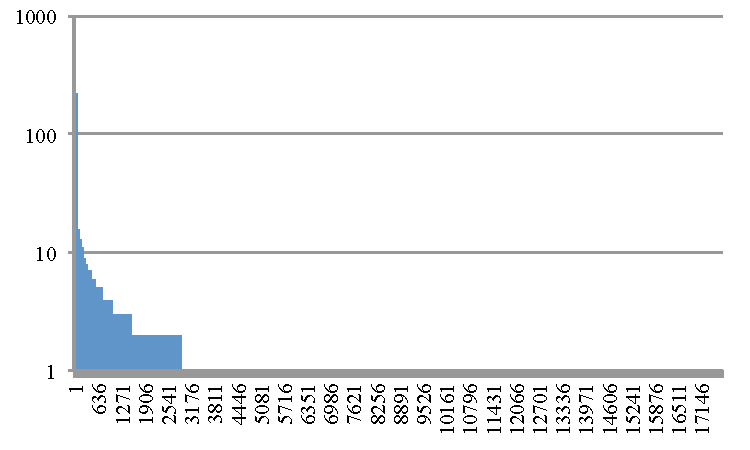
\includegraphics[clip,width=1.0\columnwidth]{images/PG_ASM}%
    \subcaption{PG (ProGuard)}\label{fig:asm-5gram-PG-histogram}%
  \end{minipage}
  \vspace{0.5cm}
  \begin{minipage}[b]{\graphwidth}
    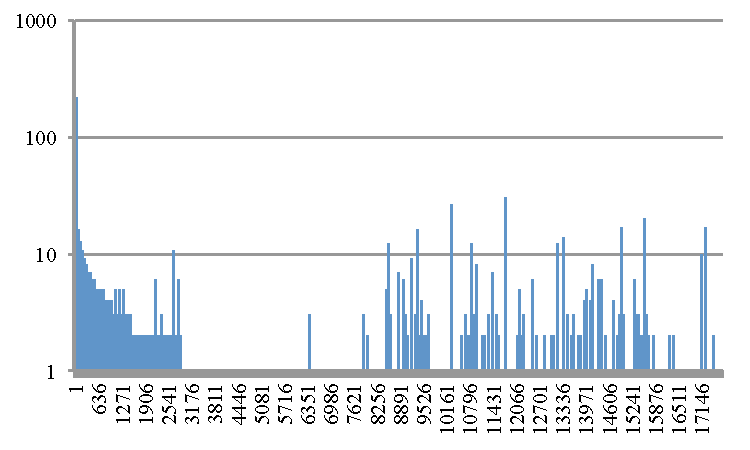
\includegraphics[clip,width=1.0\columnwidth]{images/DR_ASM}%
    \subcaption{DR (Duplication Registers)}
    \label{fig:asm-5gram-DR-histogram}%
  \end{minipage}
  \hfill
  \begin{minipage}[b]{\graphwidth}
    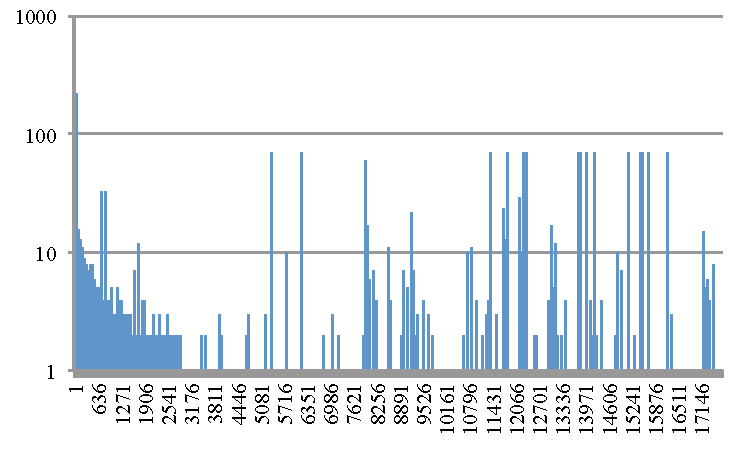
\includegraphics[clip,width=1.0\columnwidth]{images/IRR_ASM}%
    \subcaption{IRR (Irreducibility)}\label{fig:asm-5gram-IRR-histogram}%
  \end{minipage}
  \hfill
  \begin{minipage}[b]{\graphwidth}
    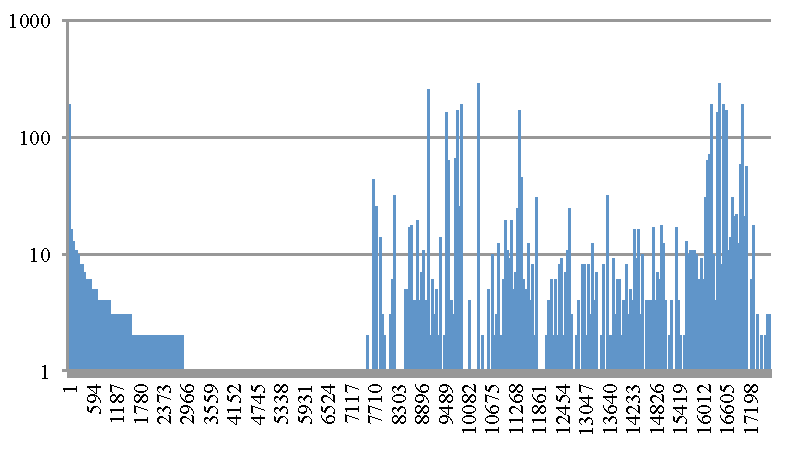
\includegraphics[clip,width=1.0\columnwidth]{images/MLI_ASM}%
    \subcaption{MLI (Merge local integers)}
    \label{fig:asm-5gram-MLI-histogram}%
  \end{minipage}
  \caption{Histogram of ASM opcdoe in 5-gram (Sorted by original 5-gram frequencies)}
  \label{fig:asm-5gram-histogram}
\end{figure*}

\begin{table}[t]
  \centering
  \footnotesize{
    \caption{Target jar files}\label{table:jars}
  \begin{tabular}{l|r||l|r}
    \textbf{Product} & \textbf{Version} & \textbf{Product} & \textbf{Version} \\ \hline
    ASM       & 3.3.1 & FakeHack  & 1.0 \\
    Jhstop    & 0.0.1 & Jwhich    & 1.0  \\
    JCalendar & 1.3.3 & Robocode-setup & 1.6.0.1  \\
  \end{tabular}
  \vspace{0.5cm}
  \caption{Obfuscation tools}\label{table:tools}
  \begin{tabular}{ll|p{4cm}}
      \textbf{Tools (Algorithms)} & \textbf{Abbr.} & \textbf{Description} \\ \hline
      Allatori Java Obfuscator\footnotemark[1] & ALL & Commercial tool. \\ \hline
      ProGurad\footnotemark[2]                 & PG  & Popular OSS obfuscation tool. \\ \hline
      Sandmark\footnotemark[3]                 &     & Academic protection tool which have many protection algorithms. \\
      \hspace{0.1cm} Duplication registers & DR & duplicate register for variables. \\
      \hspace{0.1cm} Merge local integers & MLI & merge two integer values into one long value.\\
      \hspace{0.1cm} Irreducibility       & IRR & update the control flow to irreducible one.\\
  \end{tabular}}
\end{table}

In this study, we conduct three experiments to answer the three
research questions.
\begin{description}
\item[RQ1]   What characteristics does the obfuscation method have?
\item[RQ2-1] Are the characteristics useful to identify the known
  obfuscation method applied to an unknown product?
\item[RQ2-2] Are the characteristics useful to identify the unknown
  obfuscation method applied to known product?
\end{description}
In the first experiment, we extract $n$-grams of practical protection
tools, and investigate the characteristics.
%
The second experiment tried to identify the known protection
algorithm.  The third experiment is similar with second experiment,
tried to identify the unknown protection algorithm.

To conduct the experiments, we chose the products shown in Table
\ref{table:jars}.  Also, the adopted obfuscation tools are shown in
Table \ref{table:tools}.  The first column represents tool names and
algorithm names of Sandmark.  The column named \textbf{Abbr.} shows
abbreviation of the tools and algorithms.  The last column shows short
descriptions of each tool and algorithm.
%
We conducted the experiments on the Java platform, because many
obfuscation algorithms are implemented.

Extracted characteristics are $n$-gram of opcodes, and computes their
perplexities and frequencies.  The $n$ value is 2, 3, 4, and 5.

\footnotetext[1]{\url{http://www.allatori.com}}
\footnotetext[2]{\url{http://proguard.sourceforge.net}}
\footnotetext[3]{\url{http://sandmark.cs.arizona.edu}}

At first, we constructed the corpus to compute perplexity.
Therefore, we downloaded 3,786 jar files which are distributed by the
apache software foundation\footnote[4]{\url{http://www.apache.org/}}.
Note that, the total number of classes is 660,465, and the total
number of methods is 4,272,567.

\subsection{Analysis of $n$-gram}\label{sect:rq1}

\begin{table*}[t]
  \centering
  \caption{ASM opcodes in 5-gram before/after obfuscation (top 5 frequencies)}\label{table:5gram}
  {\footnotesize
  \begin{tabular}{lc|l|r|r}
    & \textbf{Rank} & \textbf{5-gram} & \textbf{Frequency} & \textbf{Perplexity} \\ \hline
\multirow{5}{*}{{Original}}
& 1 & \verb!<code> <code> <code> <code> aload        ! &  219 & 6.12$\times10^1$ \\
& 2 & \verb!<code> <code> <code> aload getfield      ! &  122 & 6.59$\times10^2$ \\
& 3 & \verb!aload getfield ifnull aload getfield     ! &   37 & 2.48$\times10^3$ \\
& 4 & \verb!istore iload aload arraylength if_icmpge ! &   32 & 2.31$\times10^3$ \\
& 5 & \verb!aload ldc invokespecial goto aload       ! &   30 & 7.25$\times10^3$ \\ \hline
\multirow{5}{*}{{ALL}}
& 1 & \verb!aload dup getfield swap getfield               ! &  39 & 3.19$\times10^5$ \\
& 2 & \verb!aload getfield ldc invokestatic invokevirtual ! &  32 & 5.95$\times10^3$ \\
& 3 & \verb!ldc invokestatic aload invokevirtual ifeq     ! &  32 & 2.29$\times10^3$ \\
& 4 & \verb!goto ldc invokestatic aload invokevirtual     ! &  26 & 8.65$\times10^3$ \\
& 5 & \verb!dup istore iload if_icmpge aload              ! &  25 & 1.02$\times10^4$ \\ \hline
\multirow{5}{*}{{DR}}
& 1 & \verb!iconst_0 dup istore istore iload       ! & 30 & 1.08$\times10^4$ \\
& 2 & \verb!dup istore istore iload aload          ! & 27 & 3.08$\times10^4$ \\
& 3 & \verb!istore istore iload aload arraylength  ! & 20 & 8.31$\times10^4$ \\
& 4 & \verb!invokevirtual pop iconst_0 dup istore  ! & 17 & 2.27$\times10^4$ \\
& 5 & \verb!pop iconst_0 dup istore istore         ! & 17 & 1.41$\times10^4$ \\ \hline
\multirow{5}{*}{{MLI}}
& 1 & \verb!dup2X2 lxor lconst_1 lneg bipush ! & 291 & 1.13$\times10^6$ \\
& 2 & \verb!lload dup2X2 lxor lconst_1 lneg  ! & 291 & 5.37$\times10^5$ \\
& 3 & \verb!aload lload bipush lshr l2i      ! & 253 & 5.14$\times10^3$ \\
& 4 & \verb!bipush lushr land lxor lstore    ! & 187 & 5.21$\times10^4$ \\
& 5 & \verb!lconst_1 lneg bipush lushr land  ! & 187 & 9.63$\times10^4$ \\ \hline
\multirow{5}{*}{{IRR}}
& 1 & \verb!i2l iconst_0 i2l lcmp iconst_1  ! & 71 & 1.08$\times10^4$ \\
& 2 & \verb!i2l lcmp iconst_1 ixor iconst_1 ! & 71 & 3.08$\times10^4$ \\
& 3 & \verb!iconst_0 i2l lcmp iconst_1 ixor ! & 71 & 8.31$\times10^4$ \\
& 4 & \verb!iconst_1 ixor iconst_1 iand nop ! & 71 & 1.31$\times10^3$ \\
& 5 & \verb!iconst_2 irem istore iload i2l  ! & 71 & 1.47$\times10^4$ \\
  \end{tabular}}
\end{table*}

In this experiment, we try to characterize the protection methods.  At
first, we obfuscate 6 products shown in Table \ref{table:jars} by five
obfuscators shown in Table \ref{table:tools}.  Next, we extract
$n$-grams of opcode sequence from gotten 30 products and 6 original
products.  Finally, we investigate the characteristics of each tool.

The histogram of opcode frequencies is shown in the figure
\ref{fig:asm-5gram-histogram}.  The horizontal axis represents each
5-gram, and the vertical axis shows their frequencies in logarithm.
The order of the horizontal axis of all graphs is the same as original
histogram.
%
The histogram of original and PG look the same.  From investigation
of their 5-grams, both 5-grams were just the same.  We also
investigated 5-grams from other products, the result was almost the
same as 5-gram from original.  The main algorithm of PG does not
affect opcode sequences.  Therefore, the proposed method are not
useful for such obfuscation methods, which keep opcode sequences.

On the other hand, histogram of other tools is dramatically different
from original histogram.  The results show that the protection methods
may affect the opcode sequences by their characteristics.

Table \ref{table:5gram} shows 5-gram of ASM (top 5 frequencies).  On
the Table \ref{table:5gram}, we omitted PG, since just the same as
original 5-grams.  From the table \ref{table:5gram}, frequencies were
decreased except MLI, and perplexities became a quite high value.  The
result shows that obfuscated opcode sequences have rare opcode
fragments, and their fragments would be characteristics.

We found characteristics of the protection tools through investigation
of every product, shown in the Table \ref{table:characteristics}.
Unfortunately, the characteristics of PG were not found, therefore, other
identifying method is required.  Table \ref{table:characteristics} is
the answer of RQ1.

\begin{table}[t]
  \centering
  \footnotesize{
    \caption{Characteristics of the protection methods}\label{table:characteristics}
  \begin{tabular}{l|p{6.5cm}}
    \textbf{Tools} & \textbf{Characteristics for identifying} \\ \hline
    ALL  & Swap two original opcodes by \texttt{swap} instruction. \\
    PG   & Almost the same as original opcode sequence.  The proposed method cannot identify this tool. \\
    DR   & Duplicate \texttt{istore} instruction. \\
    MLI  & Emerge rare 2-gram \texttt{dup2x2 lxor}. \\
    IRR  & Emerge \texttt{nop} instruction. \\
  \end{tabular}}
\end{table}

\subsection{Identifying the known protection method}\label{sect:rq2-1}

\begin{figure}[bt]
  \centering
  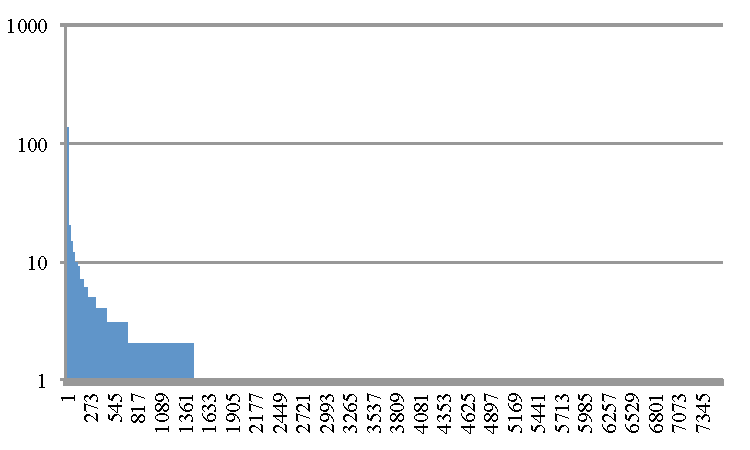
\includegraphics[width=0.32\textwidth]{images/ORI_junit}%
  \subcaption{Histogram of 5-grams from original product}\label{fig:junit-5gram-original-histogram}%
  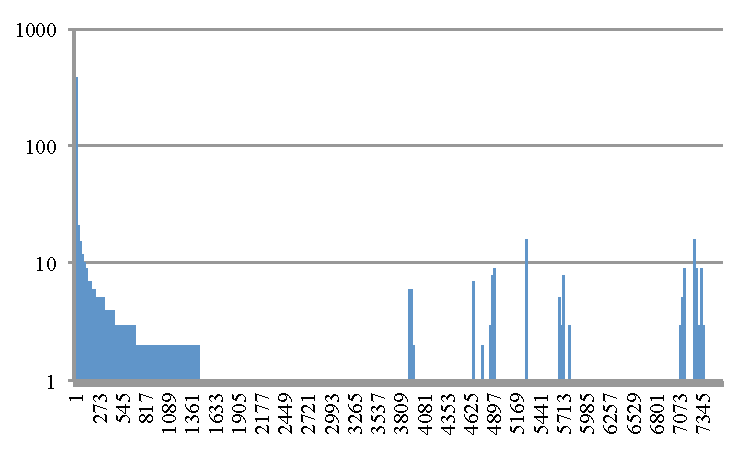
\includegraphics[width=0.32\textwidth]{images/MLI_junit}%
  \subcaption{Histogram of 5-grams from obfuscated product}\label{fig:junit-5gram-MLI-histogram}%
  \caption{Histogram of junit opcdoe in 5-gram (Sorted by original 5-gram frequencies)}
  \label{fig:junit-5gram-histogram}
\end{figure}
  
In the previous experiment, we found the characteristics of each tool.
In this experiment, we try to identify the known protection method to
the unknown products.  The known protection method means that the
characteristics were already extracted.

We chose JUnit 3.7\footnote[5]{\url{http://junit.org/}} as the unknown
product, and known protection methods are randomly selected from Table
\ref{table:tools} except PG.  Then, we obfuscated \texttt{
  junit-3.7.jar} and obtain \texttt{junit-3.7-obfuscated.jar}.
Next, we extract 5-grams from \texttt{junit-3.7-obfuscated.jar} and
computes frequencies and perplexities of 5-grams.

Figure \ref{fig:junit-5gram-original-histogram} shows histograms of
5-grams extracted from \texttt{junit-3.7.jar} and
\texttt{junit-3.7-obfuscated.jar}.  At this time, the obfuscation
algorithm was unknown, however, we suppose that some obfuscation
algorithms were applied from the graphs.  Then, we compare to the
graph of figure \ref{fig:junit-5gram-MLI-histogram} and graphs in
figure \ref{fig:asm-5gram-histogram}.  The figure
\ref{fig:junit-5gram-MLI-histogram} seems to be similar with DR
(Figure \ref{fig:asm-5gram-DR-histogram}) and MLI (Figure
\ref{fig:asm-5gram-MLI-histogram}) from the shapes of the graphs.
However, we did not succeed identifying the obfuscation method yet,
since the graph shapes are not matched exactly.

Then, we inspect the details of opcode sequences based on
characteristics of protection methods shown in Table
\ref{table:characteristics}.  Before inspection, we filtered target
5-grams as follows:
%
Let $P=\{ g_1, g_2, ..., g_l \}$ be a $n$-gram set extracted from
original opcode sequence.  Also, let $P_o=\{ g^o_1, g^o_2, ..., g^o_m
\}$ be a $n$-gram set from obfuscated opcode sequence.  Then, we
filter the 5-grams in the set difference $P_o \setminus P = \{ x
\in P_o | x \not\in P \}$.  The resultant 5-grams of top 5 frequences
are shown in Table \ref{table:junit}.  The column named \textbf{Freq.}
means frequencies of corresponding 5-gram.  Also, the column named
\textbf{PPL} shows perplexities of corresponding 5-gram.

From Table \ref{table:junit}, high perplexity 5-grams are appearing
such as including \texttt{dup2x2 lxor}.  We inspected resultant
5-grams by the characteristics shown in Table
\ref{table:characteristics}.  Then, we infer that the MLI was applied.
Finally, the proposed method succeeded to identify the obfuscation
method, since the applied obfuscation method was MLI.  Therefore, the
answer of RQ2-1 is yes.

% Not appearing n-gram are researched by n-gram that is before applied
% obfuscation.  In the result, n-gram of high frequency in five is
% reported TABLE\ref{table:junit}.  In showing the
% TABLE\ref{table:junit}, the order are called high value in perplexity
% such as dup2X2 lxor.  As the order is characteristic, we compare it
% with characteristic in five tool ( TABLE\ref{table:junit} ).  As a
% result, characteristic in applied method of obfuscation correspond
% with characteristic in method of MLI.

\begin{table}[t]
  \centering
  \footnotesize{
    \caption{5-gram of obfuscated JUnit (top 5 frequencies)}\label{table:junit}
  \begin{tabular}{l|r|r}
    \textbf{5-grams} & \rotatebox{90}{\textbf{Freq.}} & \multicolumn{1}{c}{\textbf{PPL}}\\ \hline
    \texttt{dup2x2 lxor lconst\_1 lneg bipush}   & 16 & 1.13$\times10^6$ \\
    \texttt{lload dup2x2 lxor lconst\_1 lneg}    & 16 & 5.37$\times10^5$ \\
    \texttt{bipush lushr land lxor lstore}       &  9 & 5.20$\times10^4$ \\
    \texttt{lconst\_1 leng bipush lushr land}    &  9 & 9.60$\times10^4$ \\
    \texttt{lneg bipush lushr land lxor}         &  9 & 1.37$\times10^5$ \\
  \end{tabular}}
\end{table}

\subsection{Identifying the unknown protection method}

\begin{table}[t]
  \centering
  \footnotesize{
    \caption{5-grams of obfuscated ASM}\label{table:asm}
  \begin{tabular}{l|r|r}
    \textbf{5-grams} & \rotatebox{90}{\textbf{Freq.}} & \multicolumn{1}{c}{\textbf{PPL}}\\ \hline
    \texttt{iconst\_2 irem iconst\_0 if\_icmpne aload}  & 15 & 3.76$\times10^4$ \\
    \texttt{dup dup dup imul imul}                      & 14 & 4.24$\times10^6$ \\
    \texttt{dup dup imul imul isub}                     & 14 & 8.74$\times10^5$ \\
    \texttt{dup imul imul isub iconst\_3}               & 14 & 3.49$\times10^5$ \\
    \texttt{iload dup dup dup imul}                     & 14 & 1.01$\times10^7$ \\
    \end{tabular}}
\end{table}

%%%%%% SOP手法のグラフ

\begin{figure}[b]
  \centering
  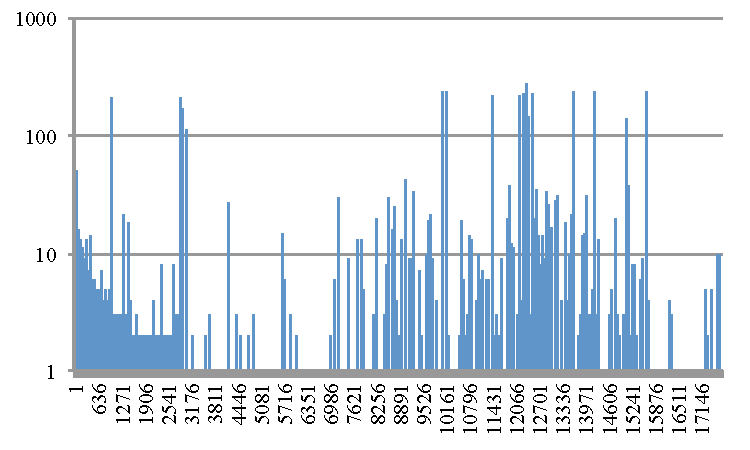
\includegraphics[clip,width=0.32\textwidth]{images/SOP_ASM}
  \caption{5-gram of obfuscated ASM with unknown algorithm}
  \label{fig:SOP}
\end{figure}

%%%%%%

%\begin{table}[t]
%  \centering
%  \footnotesize{
%    \caption{5-grams of obfuscated Jhstop}\label{table:jhstop}
%  \begin{tabular}{l|r|r}
%    \textbf{5-grams} & \textbf{Freq.} & \textbf{PPL}\\ \hline
%    \texttt{irem iconst\_0 if\_icmpne aload getfield} & 15 & 1.50$\times10^4$ \\
%    \texttt{dup dup dup imul imul}                    & 14 & 4.24$\times10^6$ \\
%    \texttt{dup dup imul imul isub}                   & 14 & 8.74$\times10^5$ \\
%    \texttt{dup imul imul isub iconst\_3}             & 14 & 3.49$\times10^5$ \\
%    \texttt{iload dup dup dup imul}                   & 14 & 1.01$\times10^7$ \\
%    \end{tabular}}
%\end{table}

In this experiment, we try to identify the unknown protection method.
The unknown protection method means that we never extract the
characteristics from it.

At first, we chose ASM 3.3.1 as the target products, and SOP (simple
opaque predicate) as the unknown protection method.  SOP is a
protection algorithm implemented in Sandmark.  SOP algorithm inserts
the opaque predicate (the \emph{if} statement always true or false)
into the programs.

At first, we obfuscated \texttt{asm-3.3.1.jar} and got
\texttt{asm-3.3.1-obfuscated.jar}.
%
Next, we obtained $n$-grams from both jar files in the same way as
Section \ref{sect:rq2-1}.  The histogram of 5-grams is shown in Figure
\ref{fig:SOP}.  The graph of figure \ref{fig:SOP} is similar with
graph of figure \ref{fig:asm-5gram-DR-histogram}.  However, the graphs
are not matched.  Therefore, we inspect the 5-grams from
\texttt{asm-3.3.1-obfuscated.jar}.

The resultant 5-grams of top 5 friequencies are shown in the Table
\ref{table:asm}, and we inspect them with the characteristics shown in
Table \ref{table:characteristics}.  From Table \ref{table:asm}, all of
5-grams have high perplexities, and include multiple \texttt{dup}, and
\texttt{imul} instructions.  The characteristics of the protection
method is not appeared in Table \ref{table:asm}.  Therefore, we cannot
identify the applied obfuscation method.
%
However, we can infer some protection method was applied since the
resultant 5-grams did not appear in original opcode sequences.
%
Naturally, we were able to identify the SOP by extracting
characteristics beforehand in the same way as Section \ref{sect:rq1}.

Therefore, the answer of RQ2-2 is no. However, extracting
characteristics from many protection methods strengthens the proposed
method.

% In this purpose, known products are obfuscated by using the unknown
% method of obfuscation, after we identify how method of obfuscation are
% used.
% 
% As a result, we analyze the RQ2-2.  
% 
% Not appearing n-gram are researched by n-gram that is before applied
% obfuscation.  In the result, n-gram of high frequency in five is
% reported TABLE\ref{table:jhstop}.  In showing the
% TABLE\ref{table:jhstop}, the order that is high value in perplexity
% are called dup and imul orders in continuous.  As the order is
% characteristic, we compare it with characteristic in five tool (
% TABLE\ref{table:jhstop} ).  As a result, characteristic in unknown
% method of obfuscation do not correspond with characteristic in
% analyzed method.
% 
% In the next, as difference product are obfuscated unknown method of
% obfuscation, we compare the each characteristic.  As a result, as the
% same characteristic are identified, we understand that unknown method
% of product is method of SOP.


\section{Conclusion}\label{sect:conclusion}

This paper proposed the method to identify the applied protection
method by artificiality evaluation method towards de-obfuscation.  We
developed three research questions to evaluate the proposed method.
In the empirical studies, we examined the proposed method to answer
the three research questions.  The answer of RQ1 is shown in the
Table \ref{table:characteristics}, the answer of RQ2-1 is yes, and the
answer of RQ2-2 is no.  However, the our method becomes useful
gradually by extracting characteristics of many protection methods
beforehand.

In this paper, the characteristics of ProGuard could not extract.  To
support such protection tools is left to our future work.  It is also
interesting research topic to identify the obfuscation method
automatically.

% In this paper, we took the identification of method of protection by
% watching the unnatural evaluation.  The actual program was applied
% method of protection and extracted characteristic to base on frequency
% and perplexity to order line of n-gram.  In this evaluation
% experiment, the identification of known obfuscation is easy and the
% identification of unknown obfuscation is difficult.  This solution
% plan is to increase the characteristic of method of obfuscation.  it
% can respond to method of unknown obfuscation by increasing
% characteristic.

% \section*{Acknowledgment}

\bibliographystyle{IEEEtran}

\bibliography{icis2016_sagisaka}

\end{document}


